% Compiled once at Docker build time to warm Tectonic's package-bundle cache into
% an image layer, so the first real compile after a cold start needs no network.
% Pulls the packages most academic papers use.
\documentclass{article}
\usepackage{amsmath,amssymb,amsthm}
\usepackage{graphicx,hyperref,geometry,xcolor,booktabs,url}
\usepackage{tikz}
\title{Warm-up}
\author{MiLatexAI}
\begin{document}
\maketitle
\section{Introduction}
Euler's identity: \(e^{i\pi} + 1 = 0\).
\begin{align}
  a &= b + c, \\
  \int_0^1 x^2 \, dx &= \tfrac{1}{3}.
\end{align}
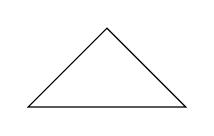
\begin{tikzpicture}
  \draw (0,0) -- (1,1) -- (2,0) -- cycle;
\end{tikzpicture}
\begin{table}[h]\centering
\begin{tabular}{lr}\toprule A & B \\ \midrule 1 & 2 \\ \bottomrule\end{tabular}
\end{table}
\end{document}
